\seite{}{Implizite Integratoren}\anchorpage{1}{neu3}{3 · Implizite Integratoren, Radau IIA und BDF}\ey{KAPITEL 3}\ptitle{Implizite Integratoren, Radau IIA und BDF}
Der schnelle Wärmeausgleich ist vorüber. Der Stab nähert sich seinem Gleichgewicht jetzt gemächlich. Trotzdem verwirft ein expliziter Solver lange Schritte. Lohnt sich eine aufwendigere Gleichung pro Schritt, wenn sie die abgeklungene Mode zuverlässig dämpft?
\subt{Der Weg durch das Kapitel}
{\tblstart\begin{tabularx}{\linewidth}{@{}Yr@{}}\toprule
\hyperlink{abs3-1}{3.1 · Stabilität in der komplexen Ebene} & \pagelink{abs3-1}\\[2pt]
\hyperlink{abs3-2}{3.2 · Nichtlineare Gleichungen im Integrationsschritt} & \pagelink{abs3-2}\\[2pt]
\hyperlink{abs3-3}{3.3 · Radau IIA aus der Kollokation} & \pagelink{abs3-3}\\[2pt]
\hyperlink{abs3-4}{3.4 · Rückwärtsdifferenzen und variable Ordnung} & \pagelink{abs3-4}\\[2pt]
\bottomrule\end{tabularx}\par}
\par\vfill{\centering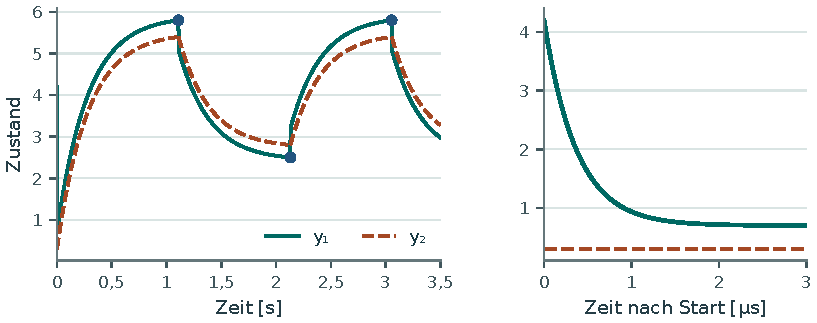
\includegraphics[width=.88\linewidth,height=49mm,keepaspectratio]{c05.pdf}\par}\capline{C05 hat auch nach dem schnellen Einschwingen eine messbare Schaltzeit.}
\seite{}{Implizite Integratoren}\anchorpage{2}{abs3-1}{3.1 · Stabilität in der komplexen Ebene}\ey{ABSCHNITT 3.1}\ptitle{Stabilität in der komplexen Ebene}
\hypertarget{punkt3-1-1}{}\subt{3.1.1\enspace Stabilitätsgebiete lesen}
Für \(y'=\lambda y\) wird aus einem Schritt die Multiplikation mit \(R(z)\), \(z=h\lambda\). Euler liefert \(1+z\). Die Randlinie \(|1+z|=1\) ist ein Kreis um \(-1\) mit Radius eins. Rückwärts-Euler löst \(y^+=y+h\lambda y^+\) und liefert \(R=1/(1-z)\). Ein imaginärer Anteil in \(\lambda\) bedeutet Rotation. Ein Abgleich nur auf der negativen reellen Achse übersieht sie.
\hypertarget{punkt3-1-2}{}\subt{3.1.2\enspace A-, Sektor- und L-Stabilität}
Eine A-stabile Einschrittmethode besitzt \(|R(z)|\le1\) auf der gesamten abgeschlossenen linken Halbebene. Bei \(A(\alpha)\)-Stabilität genügt dort ein Sektor mit Halbwinkel \(\alpha\) um die negative reelle Achse. L-Stabilität verlangt zusätzlich \(R(z)\to0\) für sehr große steife Argumente in der linken Halbebene. Die Trapezregel liefert bei \(z=-100\) den Faktor \(-49/51\), Rückwärts-Euler dagegen \(1/101\). Das Vorzeichen und die Größe erklären das numerische Nachschwingen im ersten Fall.
\notebox{Rechenfrage}{Bei welchem der beiden Ergebnisse ist die schnelle Mode nach zwei Schritten noch fast so groß wie zu Beginn? Quadrieren Sie beide Faktoren.}
\lektion{Rechenversuch · Ein steifer Folgeregler}{tracking}{Kernweg}{Zeitintegration}
Ein normierter Ausgang \(y\) soll einer Führungsgröße \(r(t)=\cos t\) folgen. Eine Vorsteuerung liefert \(\dot r\), eine Rückkopplung korrigiert den Abstand mit Rate \(a=1000\). Dadurch gilt \(\dot y=\dot r+a(r-y),\ y(0)=0\). Für den Folgefehler folgt \((y-r)'=-a(y-r)\). Somit ist \(y(t)=\cos t-e^{-1000t}\) eine unabhängige Referenz. Die Anfangsschicht dauert Millisekunden, der Versuch läuft bis \(2\unitm s\) bei \(t\) in Sekunden.

Alle Läufe verwenden dieselbe Gleichung und \(\mathrm{atol}=\mathrm{rtol}/100\). Für Radau und BDF ist \(J=[-1000]\) vorgegeben. \(E\) ist der größte Betrag des Fehlers der dichten Ausgabe auf einem gemeinsamen Gitter mit zusätzlicher Auflösung in der Anfangsschicht. Das Ziel ist \(E\le10^{-4}\).
{\tblstart\begin{tabularx}{\linewidth}{@{}Yrrrrr@{}}\toprule
\hd{Solver}&\hd{rtol}&\hd{Schritte}&\hd{\(f\)-Aufrufe}&\hd{LU}&\hd{\(E\)}\\\midrule
RK45 & \(10^{-3}\)&610&4226&0&\(1{,}19\cdot10^{-3}\)\\
RK45 & \(10^{-6}\)&731&4394&0&\(7{,}31\cdot10^{-7}\)\\
Radau & \(10^{-3}\)&14&100&28&\(2{,}02\cdot10^{-3}\)\\
Radau & \(10^{-6}\)&56&410&50&\(2{,}12\cdot10^{-5}\)\\
BDF & \(10^{-3}\)&56&144&19&\(5{,}40\cdot10^{-4}\)\\
BDF & \(10^{-6}\)&125&256&28&\(1{,}07\cdot10^{-6}\)\\\bottomrule
\end{tabularx}\par}
\subt{Wie liest man den Vergleich?}
Alle drei feinen Läufe erreichen das gemeinsame Ziel. Keiner der groben Läufe erreicht es. Der feine Radau-Lauf braucht die wenigsten angenommenen Schritte. Der feine BDF-Lauf benötigt weniger Funktionsaufrufe und Faktorisierungen als der feine Radau-Lauf. Der explizite RK45-Lauf hat den kleinsten gemessenen Fehler und die meisten Funktionsaufrufe. Die Rangfolge hängt also von der Messgröße und vom Aufwand pro Operation ab.

Die Gitterpunkte sind die Vereinigung aus \(0\), 501 logarithmischen Zeiten von \(10^{-7}\) bis \(0{,}03\) und 2001 äquidistanten Zeiten von 0 bis 2. Zwischen diesen Punkten kann der Fehler größer sein. Hier wird keine Maximalfehlergarantie und keine Laufzeitrangfolge aus den Zählern abgeleitet.
\srcs{Neu gerechneter Lehrversuch · NumPy 2.3.5, SciPy 1.17.0 · \texttt{nachrechnen.py}, Funktion \texttt{tracking}.}

\seite{}{Implizite Integratoren}\anchorpage{2}{abs3-2}{3.2 · Nichtlineare Gleichungen im Integrationsschritt}\ey{ABSCHNITT 3.2}\ptitle{Nichtlineare Gleichungen im Integrationsschritt}
\hypertarget{punkt3-2-1}{}\subt{3.2.1\enspace Das Newton-Verfahren für Stufengleichungen}
Für Rückwärts-Euler suchen wir die Nullstelle \(G(Y)=Y-y_n-hf(t_n+h,Y)\). Eine Korrektur \(\delta\) soll \(G(Y+\delta)\approx G(Y)+(I-hJ)\delta=0\) erfüllen. Lösen, addieren und neu auswerten ergibt Newton. Beim Beispiel \(y'=-y^2,y_n=h=1\) lautet die Gleichung \(Y^2+Y-1=0\). Aus \(Y=1\) folgt \(\delta=-1/3\), der neue Defekt beträgt nur noch \(1/9\).
\hypertarget{punkt3-2-2}{}\subt{3.2.2\enspace Analytische und numerische Jacobi-Matrizen}
Spalte \(j\) lässt sich über \([f(Y+\epsilon e_j)-f(Y)]/\epsilon\) annähern. Ein sehr großes \(\epsilon\) mittelt die Krümmung, ein sehr kleines verliert Ziffern durch Auslöschung. Eine analytische Ableitung lässt sich mit einem gerichteten Differenzenquotienten an mehreren Zuständen kontrollieren. Ein bekanntes Besetzungsmuster verringert die Arbeit bei großen Gittern.
\hypertarget{punkt3-2-3}{}\subt{3.2.3\enspace Modifiziertes Newton-Verfahren und LU-Wiederverwendung}
Hält man \(J\) im Schritt fest, kann der Solver \(P(I-hJ)=LU\) einmal faktorisieren. Jede Korrektur kostet dann zwei Dreieckslösungen. Das Protokoll unterscheidet Funktionsaufrufe, neue Matrizen, Faktorisierungen und Rücksetzungen. Stagniert das skalierte Residuum, wird die Matrix erneuert oder der Schritt wiederholt. Eine Änderung von \(h\) verändert die Newton-Matrix auch bei unverändertem \(J\).
\lektion{Die Algebra hinter impliziten Schritten}{algebra}{Kernweg}{Zeitintegration}
Beim Vorwärtsschritt kennen wir die Steigung am alten Zustand. Rückwärts Euler verlangt die Steigung am gesuchten neuen Zustand \(Y\). Es entsteht die Gleichung \(G(Y)=Y-y_n-hf(t_{n+1},Y)=0\). \emph{Implizit} bezeichnet hier die Zeitformel. Das zugrunde liegende Modell kann trotzdem eine explizite ODE sein.
\subt{Ein Newton-Schritt im Zahlenbeispiel}
Für \(\dot y=-y^2,\ y_n=1,\ h=0{,}1\) lautet \(G=Y+0{,}1Y^2-1\). Mit Startschätzung \(Y_0=1\) sind \(G(Y_0)=0{,}1\), \(G'(Y_0)=1{,}2\). Newton ergibt \(Y_1=1-0{,}1/1{,}2=0{,}916667\). Das neue Residuum ist etwa \(6{,}94\cdot10^{-4}\). Die positive Lösung der quadratischen Gleichung beträgt etwa \(0{,}916080\). Der exakte ODE-Wert ist \(1/1{,}1=0{,}909091\). Selbst eine bis auf Rundung gelöste Zeitformel hat noch Diskretisierungsfehler.

Bei mehreren Komponenten löst Newton \(J_G\,\Delta Y=-G\). Die \emph{LU-Zerlegung} faktorisiert die Matrix, gegebenenfalls nach Zeilenvertauschungen, in eine untere und eine obere Dreiecksmatrix. Bei gleicher Matrix können mehrere rechte Seiten mit denselben Faktoren durch Vorwärts- und Rückwärtseinsetzen gelöst werden. Die Zahl der Funktionsauswertungen und die Zahl solcher Faktorisierungen messen verschiedene Arten von Aufwand.
\subt{Wie aus Steigungen eine Kurve wird}
Eine \emph{Interpolation} wählt eine Funktion, die vorgegebene Werte an ausgewählten Punkten trifft. Für Punkte \(c_i\) ist \(\ell_j(c)=\prod_{i\ne j}(c-c_i)/(c_j-c_i)\) am Knoten \(c_j\) eins und an allen anderen Knoten null. Ein Polynom \(p(c)=\sum_j p_j\ell_j(c)\) nimmt so den Wert \(p_j\) bei \(c_j\) an. Bei der \emph{Kollokation} verlangt man von einem Ansatzpolynom, dass es die Differentialgleichung an bestimmten Knoten erfüllt. Radau IIA verwendet genau diese Idee.
\srcs{\refbk{stiff}{Hairer und Wanner, implizite Verfahren}\enspace·\enspace\see{radau}{Kollokationsrechnung für Radau IIA}.}

\seite{}{Implizite Integratoren}\anchorpage{2}{abs3-3}{3.3 · Radau IIA aus der Kollokation}\ey{ABSCHNITT 3.3}\ptitle{Radau IIA aus der Kollokation}
\hypertarget{punkt3-3-1}{}\subt{3.3.1\enspace Gauß-, Radau- und Lobatto-Knoten}
Eine Ersatzkurve soll an ausgewählten Punkten der Modellgleichung folgen. Gauß-Knoten liegen im Inneren, bei Radau ist ein Randpunkt enthalten, bei Lobatto beide. Für die rechte Radau-Variante ist die letzte Stufe eine Rechnung am Schrittende. Ihre Lage und die Gewichte bestimmen gemeinsam das Verhalten bei einer Bindung.
\hypertarget{punkt3-3-2}{}\subt{3.3.2\enspace Drei Stufen, fünfte Ordnung}
Für \(r=\sqrt6\) sind \(c_1=(4-r)/10, c_2=(4+r)/10, c_3=1\). Zu diesen Knoten seien \(\ell_j\) die Lagrange-Basispolynome. Integrieren der interpolierten Ableitung liefert \(a_{ij}=\int_0^{c_i}\ell_j(s)\,ds\), \(b_j=\int_0^1\ell_j(s)\,ds\). Das Tableau lautet
\[
\begin{array}{c|ccc}
c_1&(88-7r)/360&(296-169r)/1800&(-2+3r)/225\\
c_2&(296+169r)/1800&(88+7r)/360&(-2-3r)/225\\
1&(16-r)/36&(16+r)/36&1/9\\\hline
 &(16-r)/36&(16+r)/36&1/9
\end{array}
\]
Die Radau-Quadratur mit drei Knoten integriert Polynome bis Grad vier exakt. Die zugehörige Kollokationsmethode hat für hinreichend glatte ODEs globale Ordnung fünf.
\hypertarget{punkt3-3-3}{}\subt{3.3.3\enspace Stiff Accuracy und algebraische Bindungen}
Da \(a_{3j}=b_j\), ist der berechnete Endwert exakt der letzten Stufe gleich. Dies heißt \emph{stiffly accurate}. Eine in der Stufe gelöste Bindung geht damit bis zur Lösertoleranz in den Endwert ein. Eine Endstufe bei \(c_s=1\) allein garantiert das Gleichsetzen der Gewichte noch nicht. Die zugrunde liegende DAE muss regulär und passend initialisiert sein.
\lektion{Radau IIA aus einer Kollokationsidee}{radau}{Vertiefung}{Zeitintegration}
Können wir eine Kurve für den ganzen Schritt suchen und ihre Steigung an mehreren Stellen prüfen? Das dreistufige Radau-IIA-Verfahren wählt ein Polynom \(p\) vom Grad höchstens drei auf \([t_n,t_n+h]\) mit \(p(t_n)=y_n\). An den drei Prüfstellen muss die Steigung des Polynoms die Modellgleichung erfüllen.
\[
 p'(t_n+c_i h)=f(t_n+c_i h,p(t_n+c_i h)),\quad
 c_{1,2}=(4\mp\sqrt 6)/10,\quad c_3=1 .
\]
Interpolieren die Lagrange-Polynome \(\ell_j\) auf diesen drei Knoten die Stufensteigungen, so liefert Integration \(a_{ij}=\int_0^{c_i}\ell_j(s)\dg s\) und \(b_j=\int_0^1\ell_j(s)\dg s\). Weil \(c_3=1\), ergibt die letzte Stufe bereits den Endzustand. Diese Eigenschaft heißt \emph{stiffly accurate}. Das klassische dreistufige Verfahren besitzt für glatte ODEs globale Ordnung 5.
\subt{Dämpfung am Testproblem}
Für dieses Radau-Verfahren ist die Stabilitätsfunktion
\[
 R(z)=\frac{1+\frac25z+\frac1{20}z^2}
 {1-\frac35z+\frac3{20}z^2-\frac1{60}z^3}.
\]
Das Verfahren ist A-stabil. Der höhere Nennergrad erklärt darüber hinaus den Grenzwert null und damit die L-Stabilität. Bei \(z=-10\) liefert Radau \(0{,}05172\), rückwärts Euler \(0{,}09091\) und die Trapezregel \(-0{,}66667\). Die exakte Verstärkung beträgt \(e^{-10}=0{,}0000454\). Ein stabiler großer Schritt kann also für eine interessierende Anfangsschicht immer noch zu grob sein.
\subt{Wofür bezahlt man?}
Die unbekannten Stufen \(Y_i=y_n+h\sum_j a_{ij}f_j\) sind gekoppelt. Newton-Schritte verwenden Blöcke vom Typ \(\delta_{ij}I-h a_{ij}J_j\) mit \(J_j=\partial f/\partial y\). Lineare Algebra, Skalierung und Wiederverwendung von Faktorisierungen beeinflussen die Kosten. Bei großen räumlichen Gittern macht die dünn besetzte Jacobi-Matrix einen wesentlichen Unterschied.
\notebox{Implementierung}{SciPys \texttt{Radau} integriert eine ODE in der Form \(\dot y=f(t,y)\). Für eine allgemeine Residual-DAE braucht man eine Schnittstelle, die \(F(t,y,\dot y)=0\) entgegennimmt. Diese Unterscheidung wird auf S.\,\pagelink{indexeins} durchgerechnet.}
\srcs{\refbk{stiff}{Hairer und Wanner} · \refbk{scipy}{SciPy Radau} · \refbk{radtab}{Koeffizienten und Stabilitätsfunktion}.}

\seite{}{Implizite Integratoren}\anchorpage{2}{abs3-4}{3.4 · Rückwärtsdifferenzen und variable Ordnung}\ey{ABSCHNITT 3.4}\ptitle{Rückwärtsdifferenzen und variable Ordnung}
\hypertarget{punkt3-4-1}{}\subt{3.4.1\enspace BDF1 bis BDF6 konstruieren}
Der Integrator besitzt bereits frühere Zustände. Legen wir ein Polynom durch den gesuchten neuen Wert und \(k\) frühere Werte und differenzieren es am neuen Ende, entsteht bei konstantem Schritt \(h f_{n+1}=\sum_{j=0}^k\alpha_j y_{n+1-j}\). Die folgende Tabelle gibt die Zähler in zeitlich rückwärts laufender Reihenfolge an. Division durch den letzten Spaltenwert ergibt alle \(\alpha_j\).
{\tblstart\begin{tabularx}{\linewidth}{@{}rYr@{}}\toprule
\hd{Ordnung}&\hd{Zähler ab dem neuen Zustand}&\hd{Teiler}\\\midrule
1&1, \ensuremath{-}1&1\\2&3, \ensuremath{-}4, 1&2\\3&11, \ensuremath{-}18, 9, \ensuremath{-}2&6\\4&25, \ensuremath{-}48, 36, \ensuremath{-}16, 3&12\\5&137, \ensuremath{-}300, 300, \ensuremath{-}200, 75, \ensuremath{-}12&60\\6&147, \ensuremath{-}360, 450, \ensuremath{-}400, 225, \ensuremath{-}72, 10&60\\\bottomrule\end{tabularx}\par}
Setzen Sie eine konstante Kurve ein. Jede Zeilensumme ergibt null. Setzen Sie danach eine Gerade ein. Die Formel muss ihre Steigung liefern. Variable Schrittweiten erfordern neu bestimmte Differenzengewichte.
\hypertarget{punkt3-4-2}{}\subt{3.4.2\enspace Dahlquist-Barrieren und Ordnungswechsel}
Für ein konvergentes A-stabiles lineares Mehrschrittverfahren ist die Ordnung höchstens zwei. BDF1 und BDF2 sind A-stabil, die Ordnungen drei bis sechs besitzen kleinere Stabilitätssektoren. Ab BDF7 scheitert bereits die Nullstabilität der klassischen konstanten Schrittfolge. Ein adaptiver Solver vergleicht Fehler- und Kostenschätzungen benachbarter Ordnungen. Er braucht genügend glatte Historie, um höher zu schalten. Ein Stoß erzwingt deren Neustart. Die SciPy-Implementierung nutzt die Ordnungen eins bis fünf.
\srcs{\href{https://docs.scipy.org/doc/scipy/reference/generated/scipy.integrate.BDF.html}{SciPy BDF} · \refbk{ode}{Hairer, Nørsett und Wanner}.}
\lektion{Wie BDF, ESDIRK und Rosenbrock einen Schritt berechnen}{bdf}{Vertiefung}{Zeitintegration}
\subt{BDF2 verwendet einen früheren Zustand}
Eine BDF (Backward Differentiation Formula) approximiert die neue Steigung mit zurückliegenden Werten. Die Ableitung des quadratischen Interpolationspolynoms durch \(y_{n-1},y_n,y_{n+1}\) am neuen Zeitpunkt ergibt bei konstanter Schrittweite
\[
 \frac{3y_{n+1}-4y_n+y_{n-1}}{2h}=f(t_{n+1},y_{n+1}).
\]
Für \(y'=-ay\) wird daraus \((3+2ha)y_{n+1}=4y_n-y_{n-1}\). Bei einem nichtlinearen Modell muss pro Schritt eine nichtlineare Gleichung gelöst werden. Das Verfahren nutzt die Vorgeschichte. Ein Starter, etwa rückwärts Euler, erzeugt den fehlenden Anfangswert. Nach einem Zustandsreset muss die Historie passend neu aufgebaut werden.

BDF1 und BDF2 sind A-stabil. Höhere klassische BDF-Ordnungen besitzen eingeschränkte Stabilitätssektoren. Produktionssolver variieren Ordnung und Schrittweite. Für glatte lange Abschnitte kann sich diese Historie lohnen. Bei häufigen Neustarts oder genauer Ereigniszeit lohnt ein Vergleich mit Radau.
\subt{ESDIRK löst die Stufen nacheinander}
Beim explizit gestarteten, einfach diagonalen impliziten RK-Verfahren ist die erste Stufe explizit, die folgenden haben denselben Diagonalkoeffizienten \(\gamma\). Die untere Dreiecksstruktur erlaubt nacheinander kleinere nichtlineare Lösungen. Bei vereinfachtem Newton und festgehaltener Jacobi-Matrix lässt sich \(I-h\gamma J\) innerhalb eines Schritts wiederverwenden. Das eingebettete ESDIRK-3(2)-Paar der Studie kombiniert diese Struktur mit einer Fehlerkontrolle.
\subt{Rosenbrock linearisiert bereits im Verfahren}
Beim Rosenbrock--Euler-Schritt eines autonomen Systems löst man \((I-hJ_n)k=f(y_n)\) und setzt \(y_{n+1}=y_n+hk\). Das ist eine Linearisierung des impliziten Euler-Schritts und bei linearem \(f\) exakt dessen Schritt. Mehrstufige Rosenbrock-Verfahren erreichen höhere Ordnung. Sie sind Kandidaten für steife ODEs mit gut zugänglichem \(J\), besonders wenn eine nichtlineare Stufeniteration teuer wäre.
\notebox{Vergleichsmaß}{Gezählt werden angenommene Schritte, Auswertungen von \(f\), Jacobi-Matrizen und LU-Faktorisierungen. Ein einziges dichtes lineares System kann mehr kosten als viele Auswertungen eines lokalen Flusses.}
\srcs{\refbk{stiff}{Hairer und Wanner} · \refbk{esdirk}{Kværnø, eingebettete ESDIRK-Paare} · \refbk{ida}{BDF beim Residualsolver IDA}.}
\lektion{Der implizite Schritt am Newton-Protokoll}{alg3}{Werkstatt}{Kapitel 3}
Ein Newton-Schritt liefert eine Korrektur, ein Integrationsschritt einen neuen Zeitpunkt. Beide dürfen nicht verwechselt werden. Das Schema verwendet eine feste Näherung der Jacobi-Matrix pro Versuch.
{\small\begin{verbatim}
Y = Praediktor(t, y, h)
M = I - h * Jacobi(t + h, Y)
P, L, U = faktorisiere(M)
wiederhole:
    G = Y - y - h * f(t + h, Y)
    wenn Defekt_und_Korrektur_klein: beende_Iteration
    delta = loese_mit_LU(P, L, U, -G)
    Y = Y + delta
bei Stagnation: Matrix erneuern oder h verkleinern
\end{verbatim}}
\subt{Selbst rechnen}
Für den impliziten Schritt bei \(y'=-y^2\) und h=y=1 sei die Ableitung am Start festgehalten. Welcher zweite Näherungswert entsteht?
\notebox{Lösung}{Nach der ersten Korrektur ist Y=2/3 und der Defekt 1/9. Die feste Matrix ist 3. Also folgt Y=2/3\ensuremath{-}1/27=17/27. Ein frisch differenzierender Newton-Schritt würde die Matrix 7/3 benutzen. Vergleichen Sie die Defekte beider Werte mit dem exakten positiven Zielwert (\(\sqrt5\)\ensuremath{-}1)/2.}
